\documentclass[../DoAn.tex]{subfiles}
\begin{document}


\section{Khảo sát hiện trạng}


\subsection{Tổng quan các giao thức DeFi lending hiện có}


Trong hệ sinh thái DeFi, hai giao thức vay và cho vay phi tập trung có ảnh hưởng lớn và được nghiên cứu rộng rãi nhất là Compound và Aave. Cả hai đều sử dụng mô hình pool thanh khoản chung, trong đó người dùng gửi tài sản vào một pool được quản lý bởi smart contract để nhận lãi suất, và người vay có thể rút tài sản từ pool với điều kiện thế chấp tài sản khác có giá trị vượt mức khoản vay. Lãi suất trong các giao thức này được điều chỉnh tự động dựa trên tỷ lệ sử dụng vốn của từng pool: khi tỷ lệ sử dụng cao, lãi suất tăng để thu hút thêm người gửi và khuyến khích người vay trả nợ; khi tỷ lệ sử dụng thấp, lãi suất giảm để kích thích vay.

Compound ra mắt năm 2018 và là giao thức đặt nền móng cho toàn bộ lĩnh vực DeFi lending. Compound giới thiệu khái niệm lãi suất thuật toán và vị thế gửi tiền được token hóa (cToken), trở thành chuẩn mực mà Aave và các giao thức khác xây dựng theo. Về mặt kỹ thuật, khi người dùng gửi tài sản, họ nhận lại cToken tương ứng (ví dụ cUSDC). Số dư cToken không thay đổi theo thời gian, thay vào đó tỷ giá chuyển đổi giữa cToken và tài sản gốc tăng dần khi lãi tích lũy. Cơ chế kiểm soát rủi ro tập trung vào smart contract Comptroller --- đây là bộ máy quản lý rủi ro trung tâm, mọi hành động gửi, vay, rút đều phải thông qua Comptroller để kiểm tra mức thế chấp và tình trạng nợ. Compound v2 sử dụng Comptroller chung để quản lý rủi ro cho tất cả tài sản, dẫn đến rủi ro lan truyền ở tầng quản trị thế chấp: nếu một tài sản rủi ro cao bị định giá sai hoặc bị khai thác, toàn bộ hệ thống có thể bị ảnh hưởng. Compound v3 (Comet) giải quyết vấn đề này bằng cách tách thành các market độc lập, mỗi market chỉ cho phép vay một loại tài sản duy nhất trong khi vẫn chấp nhận nhiều loại collateral khác nhau, đánh đổi tính linh hoạt lấy sự an toàn và cô lập rủi ro.~\cite{CompoundWhitepaper,CompoundV2Docs,CompoundIIIDocs}.

Aave ra mắt công khai năm 2020 và phát triển qua hai thế hệ chính. Aave v2 tập trung tối ưu hóa mô hình thế chấp và lãi suất ổn định. Aave v3 bổ sung các tính năng nâng cao về hiệu quả vốn và khả năng đa chuỗi: Isolation Mode giới hạn các tài sản rủi ro cao vào các pool độc lập để ngăn ảnh hưởng hệ thống; E-Mode cho phép hệ số thế chấp rất cao với các tài sản tương quan chặt; Portal cho phép dịch chuyển thanh khoản giữa các chuỗi. Về cơ chế ghi nhận vị thế, Aave sử dụng aToken --- token mang lãi suất được mint 1:1 với tài sản gửi và số dư aToken tăng trực tiếp theo thời gian khi lãi tích lũy, khác với cToken của Compound dùng tỷ giá quy đổi. Aave còn tiên phong với Flash Loan --- cơ chế vay không cần thế chấp với điều kiện hoàn trả trong cùng một giao dịch, mở ra khả năng arbitrage, hoán đổi thế chấp và thanh lý phức tạp mà Compound không hỗ trợ~\cite{AaveV2Whitepaper,AaveV3TechPaper}.

Về mô hình lãi suất, cả Aave và Compound v2 đều áp dụng mô hình Two-Slope (còn gọi là Kinked Rate Model): lãi suất vay tăng tuyến tính theo tỷ lệ sử dụng vốn khi dưới ngưỡng tối ưu (U\_optimal), và tăng với độ dốc lớn hơn nhiều khi vượt ngưỡng này. Hai giao thức có cùng cơ chế kinh tế nhưng khác nhau về chi tiết triển khai và các tham số cấu hình~\cite{CompoundV2Docs,AaveV2Whitepaper}.

\subsection{Phân tích ưu và nhược điểm}


Bảng~\ref{table:2.1} dưới đây tổng hợp so sánh các đặc điểm kỹ thuật chính của hai giao thức tham chiếu và giao thức được xây dựng trong đồ án này:

\begin{table}[H]
\centering
\resizebox{\textwidth}{!}{%
\begin{tabular}{|p{0.22\textwidth}|p{0.25\textwidth}|p{0.27\textwidth}|p{0.27\textwidth}|}
\hline
\textbf{Tiêu chí} & \textbf{Compound v2} & \textbf{Aave v2/v3} & \textbf{Giao thức đồ án} \\ \hline
Mô hình pool & Pool chung đa tài sản & Pool chung đa tài sản (v2), Isolated (v3) & Pool chung đa tài sản \\ \hline
Ghi nhận vị thế gửi & cToken (tỷ giá quy đổi tăng dần) & aToken (số dư tăng trực tiếp) & Internal (ghi nhận bên trong smart contract) \\ \hline
Mô hình lãi suất & Two-Slope (JumpRateModel) & Two-Slope (DefaultReserve InterestRateStrategy) & Two-Slope \\ \hline
Cơ chế thanh lý & Close factor + liquidation incentive & Close factor + liquidation bonus & Close factor + liquidation incentive \\ \hline
Oracle giá & Chainlink + Uniswap TWAP & Chainlink + dự phòng & Chainlink + MyOracle (môi trường kiểm thử) \\ \hline
Nâng cấp smart contract & Proxy pattern & UUPS/Transparent Proxy & UUPS \\ \hline
Quản trị & COMP token + Timelock & AAVE token + Timelock & Multisig + ProtocolTimelock \\ \hline
Flash Loan & Không hỗ trợ & Hỗ trợ & Ngoài phạm vi \\ \hline
Đa chuỗi & Hạn chế & Hỗ trợ 14+ chuỗi & Ngoài phạm vi \\ \hline
Hệ thống backend & Outsource indexer (The Graph) + API server & Outsource indexer (The Graph) + API server & Tự xây indexer, event-driven đa tiến trình \\ \hline
\end{tabular}
}
\caption{So sánh các giao thức tham chiếu và giao thức đồ án}
\label{table:2.1}
\end{table}


Nhận xét về ưu điểm của các giao thức tham chiếu: Compound v2 nổi bật bởi sự đơn giản và rõ ràng trong thiết kế --- mô hình cToken dễ hiểu, kiến trúc Comptroller tập trung hóa quản lý rủi ro, và toàn bộ codebase đã được kiểm toán và kiểm chứng qua nhiều năm vận hành thực tế. Aave v2 cân bằng tốt giữa tính năng phong phú và độ phức tạp có kiểm soát, với hệ thống sự kiện (event) được thiết kế chi tiết cho phép tái tạo trạng thái từ lịch sử. Aave v3 đẩy giới hạn về hiệu quả vốn và khả năng mở rộng đa chuỗi, nhưng đánh đổi bằng độ phức tạp cài đặt tăng đáng kể.

Nhận xét về hạn chế liên quan đến mục tiêu đồ án: Trong thực tế, cả Aave và Compound đều phải dựa vào dịch vụ indexer bên ngoài như The Graph để phục vụ frontend với dữ liệu lịch sử và tổng hợp, tạo ra một điểm phụ thuộc vào bên thứ ba nằm ngoài kiến trúc on-chain. Đây là điểm mà đồ án này tiếp cận khác biệt: thay vì outsource indexing layer, hệ thống tự xây toàn bộ backend event-driven để chủ động kiểm soát dữ liệu và không phụ thuộc vào hạ tầng bên ngoài. Ngoài ra, tài liệu hướng dẫn xây dựng một giao thức tương tự từ đầu vẫn còn rời rạc, chưa có nguồn tham chiếu toàn diện nào trình bày đầy đủ cả ba tầng smart contract, backend và frontend trong một hệ thống thống nhất.

\subsection{Định vị của đồ án}


Từ quá trình khảo sát trên, đồ án này xác định hướng xây dựng một giao thức lending phi tập trung ở quy mô phù hợp để có thể hiểu và triển khai hoàn chỉnh, lấy thiết kế của Compound v2 và Aave v2 làm tham chiếu cho lớp smart contract~\cite{CompoundV2Docs,AaveV2Whitepaper}, tự xây toàn bộ indexing layer thay vì outsource ra The Graph, đồng thời tích hợp luôn notification và snapshot vào cùng một hệ thống backend thống nhất. Về cơ chế ghi nhận vị thế, đồ án áp dụng Global Interest Index tương tự Compound v2 nhưng lưu trực tiếp trong storage của LendingPool thay vì thông qua cơ chế token trung gian như cToken hay aToken, đơn giản hóa kiến trúc trong khi vẫn đảm bảo tính chính xác về mặt toán học. Về quản trị, đồ án áp dụng mô hình Multisig Wallet kết hợp Timelock ở quy mô nhỏ phù hợp với giai đoạn phát triển ban đầu của giao thức. Chi tiết về các quyết định thiết kế này sẽ được trình bày trong Chương~\ref{chapter:SystemDesign} và Chương~\ref{chapter:Solutions}.

Giao thức đồ án không hướng đến cạnh tranh về quy mô hay tính năng với Compound và Aave. Giá trị khác biệt nằm ở việc xây dựng và phân tích từng thành phần kỹ thuật từ đầu, bao gồm cả tầng backend thường bị bỏ qua trong các tài liệu học thuật về DeFi.

\section{Tổng quan chức năng}


Hệ thống vay và cho vay phi tập trung được thiết kế xoay quanh các tác nhân chính sau:

Người dùng (User) là tác nhân trung tâm của hệ thống. Người dùng tương tác với giao thức thông qua ví điện tử (MetaMask hoặc các ví tương thích EVM), không cần đăng ký tài khoản truyền thống. Các chức năng chính của User bao gồm: (i) Kết nối và ngắt kết nối ví điện tử, (ii) Xác thực địa chỉ và đăng nhập bằng chữ ký điện tử, (iii) Gửi tài sản vào giao thức để nhận lãi, (iv) Vay tài sản dựa trên tài sản thế chấp, (v) Trả nợ vay và rút tài sản đã gửi, (vi) Tham gia thanh lý các vị thế không đảm bảo, (vii) Theo dõi trạng thái vị thế (collateral, debt, health factor), (viii) Theo dõi các thông số tài sản đang có trong giao thức, (ix) Xem lịch sử giao dịch và các sự kiện liên quan đến tài khoản, (x) Xem các hành động của admin đối với giao thức và (xi) Đăng ký email để nhận thông báo về các thay đổi quan trọng của giao thức.

Điểm quan trọng khác với mô hình tiết kiệm ngân hàng truyền thống, giao thức không ràng buộc người dùng vào kỳ hạn cố định. Người dùng có thể gửi tài sản và rút ra bất kỳ lúc nào, đồng thời vẫn nhận đủ lãi suất tương ứng với thời gian thực tế đã gửi tính đến giây. Tương tự, lãi suất vay và gửi không cố định mà thay đổi liên tục theo tỷ lệ sử dụng vốn của từng tài sản trong giao thức. Hai tính chất này --- không kỳ hạn và lãi suất thả nổi --- là yêu cầu cốt lõi quyết định toàn bộ cách thiết kế cơ chế tích lũy lãi của hệ thống.

Admin là tác nhân có quyền quản trị hệ thống, kế thừa toàn bộ chức năng của User. Ngoài ra, Admin còn có các quyền đặc biệt nhằm đảm bảo hoạt động ổn định và an toàn của giao thức (tất cả các hành động của admin đều được thực hiện thông qua ví đa chữ ký và timelock), bao gồm: (i) Quản lý danh sách tài sản được hỗ trợ, (ii) Cấu hình các tham số của giao thức (lãi suất, hệ số thế chấp, ngưỡng thanh lý,…), (iii) Tạm dừng hoặc kích hoạt lại giao thức trong trường hợp khẩn cấp, (iv) Quản lý các hợp đồng thông minh liên quan đến giao thức (update địa chỉ, logic (với những upgradeable contract)), (v) Quản lý ngân quỹ và các hoạt động tài chính của giao thức.

Oracle là tác nhân hệ thống bên ngoài, có nhiệm vụ cung cấp dữ liệu giá tài sản on-chain cho giao thức. Trong đồ án, Chainlink Data Feed được sử dụng nhằm đảm bảo dữ liệu giá có độ tin cậy cao, chống thao túng và phù hợp với yêu cầu của các ứng dụng DeFi~\cite{ChainlinkDocs}.

\subsection{Biểu đồ usecase tổng quát}


Sơ đồ ca sử dụng tổng quát của hệ thống được thể hiện bởi hình~\ref{fig:uctq} dưới đây

\begin{figure}[H]
\centering
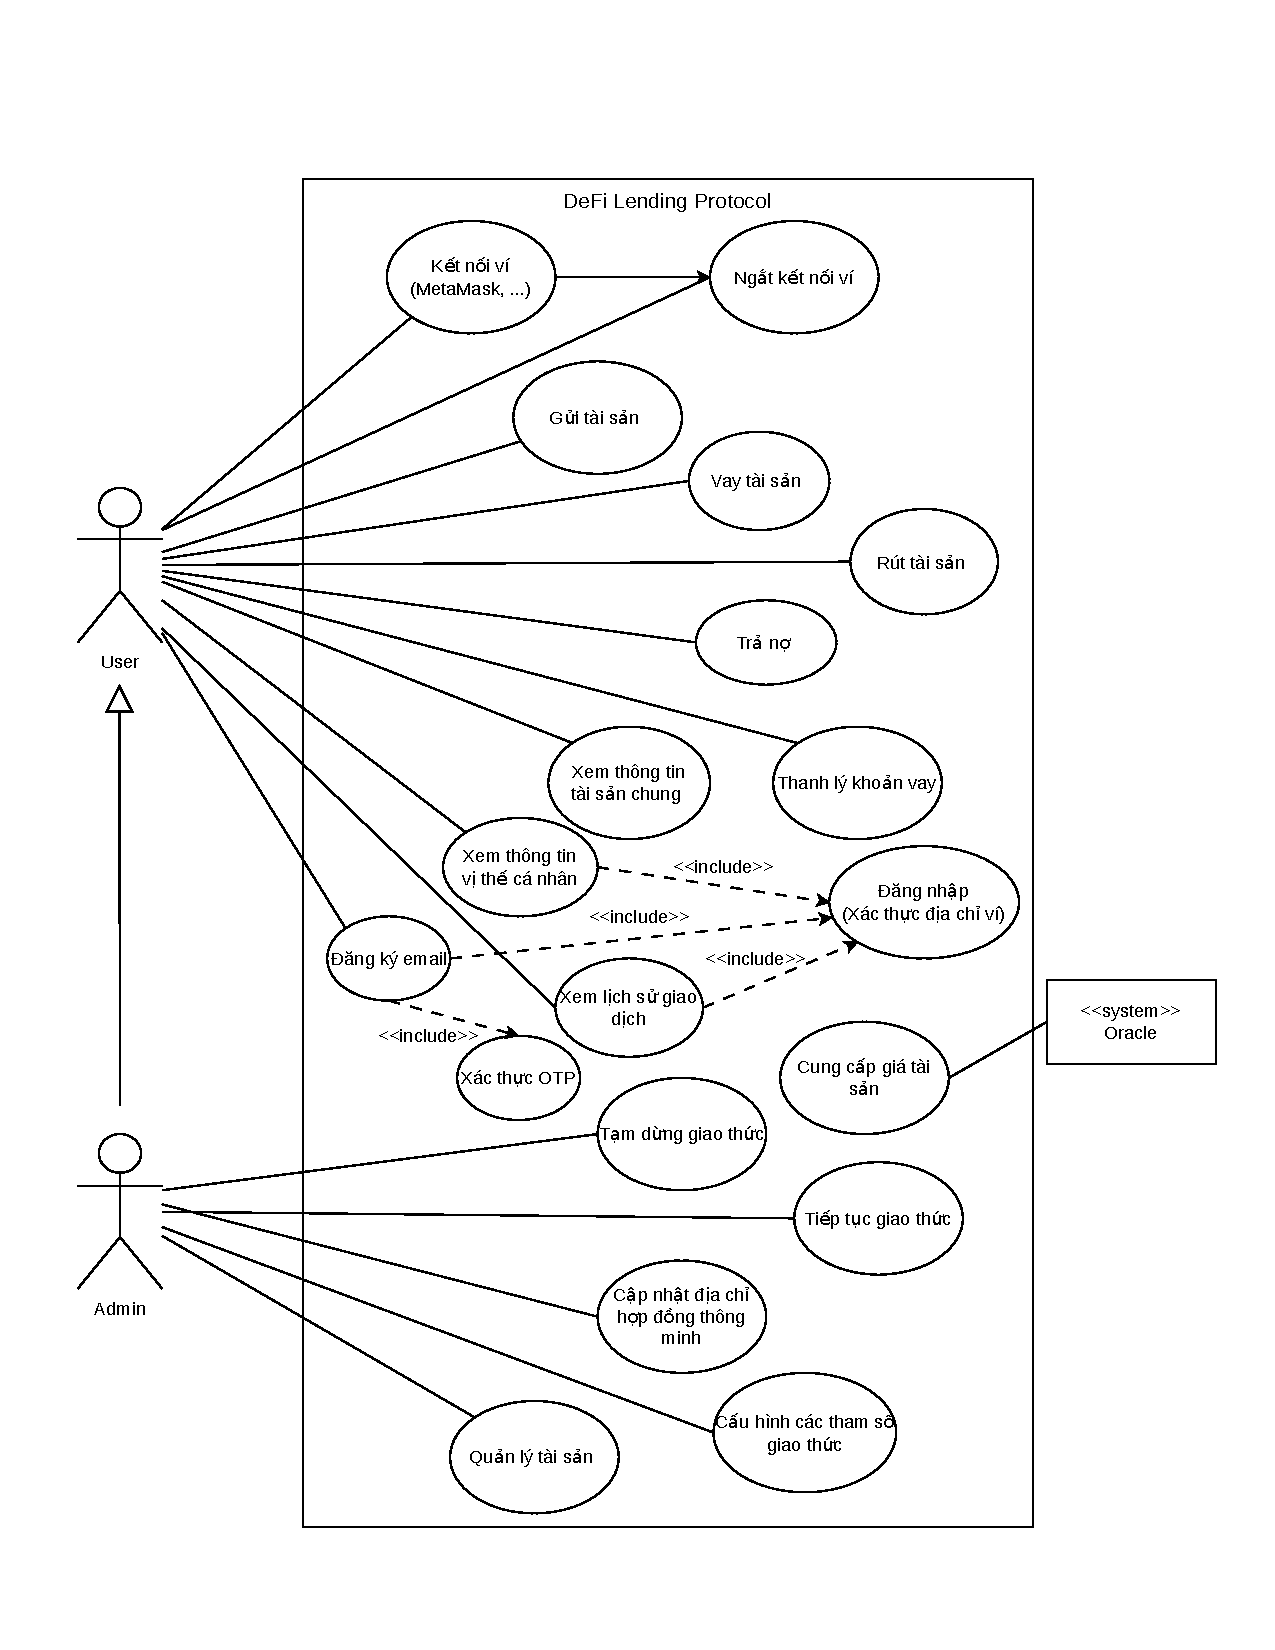
\includegraphics[
    page=1,
    width=\textwidth,
    height=0.9\textheight,
    keepaspectratio
]{../Hinhve/UCTQ.pdf}
\caption{Sơ đồ usecase tổng quát}
\label{fig:uctq}
\end{figure}

\subsection{Biểu đồ usecase phân rã}


Sơ đồ ca sử dụng phân rã quản lý tài sản được thể hiện bằng hình~\ref{fig:ucpr} dưới đây

\begin{figure}[H]
\centering
\includegraphics[width=0.9\textwidth]{Hinhve/UCPR.png}
\caption{Sơ đồ usecase phân rã quản lý tài sản}
\label{fig:ucpr}
\end{figure}


\section{Đặc tả chức năng}


\subsection{Kết nối ví}


Đặc tả usecase kết nối ví được thể hiện bằng hình~\ref{fig:dtknv}, sơ đồ tuần tự được thể hiện trong hình~\ref{fig:ssdknv}

\begin{figure}[H]
\centering
\includegraphics[
    page=1,
    width=\textwidth,
    height=0.9\textheight,
    keepaspectratio
]{Hinhve/DTKNV.pdf}
\caption{Đặc tả usecase Kết nối ví}
\label{fig:dtknv}
\end{figure}


\begin{figure}[H]
\centering
\includegraphics[
    page=1,
    width=\textwidth,
    height=0.9\textheight,
    keepaspectratio
]{Hinhve/SSDKNV.pdf}
\caption{Sơ đồ tuần tự Kết nối ví}
\label{fig:ssdknv}
\end{figure}


\subsection{Đăng nhập (Xác thực địa chỉ ví)}


Đặc tả usecase đăng nhập (Xác thực địa chỉ ví) được thể hiện bằng hình~\ref{fig:dtdn}, sơ đồ tuần tự được thể hiện trong hình~\ref{fig:ssddn} dưới đây

\begin{figure}[H]
\centering
\includegraphics[
    page=1,
    width=\textwidth,
    height=0.9\textheight,
    keepaspectratio
]{Hinhve/DTDN.pdf}
\caption{Đặc tả usecase Đăng nhập (Xác thực địa chỉ ví)}
\label{fig:dtdn}
\end{figure}


\begin{figure}[H]
\centering
\includegraphics[
    page=1,
    width=\textwidth,
    height=0.9\textheight,
    keepaspectratio
]{Hinhve/SSDDN.pdf}
\caption{Sơ đồ tuần tự Đăng nhập (Xác thực địa chỉ ví)}
\label{fig:ssddn}
\end{figure}


\subsection{Gửi tài sản}


Đặc tả usecase Gửi tài sản được thể hiện bằng hình~\ref{fig:dtgts}, cùng với sơ đồ tuần tự trong hình~\ref{fig:ssdgts} dưới đây

\begin{figure}[H]
\centering
\includegraphics[
    page=1,
    width=\textwidth,
    height=0.9\textheight,
    keepaspectratio
]{Hinhve/DTGTS.pdf}
\caption{Đặc tả usecase Gửi tài sản}
\label{fig:dtgts}
\end{figure}


\begin{figure}[H]
\centering
\includegraphics[
    page=1,
    width=\textwidth,
    height=0.9\textheight,
    keepaspectratio
]{Hinhve/SSDGTS.pdf}
\caption{Sơ đồ tuần tự Gửi tài sản}
\label{fig:ssdgts}
\end{figure}


Đối với các ca sử dụng Vay tài sản, Trả nợ và Rút tài sản, ba chức năng còn lại của nghiệp vụ cốt lõi (Vay --- Borrow, Trả nợ --- Repay, Rút --- Withdraw) có chung mô hình tương tác với Gửi tài sản: người dùng nhập số tiền trên giao diện $\rightarrow$ frontend gọi MetaMask để ký giao dịch (bao gồm bước approve ERC-20 nếu cần) $\rightarrow$ MetaMask broadcast giao dịch lên blockchain $\rightarrow$ smart contract thực thi nghiệp vụ và phát event $\rightarrow$ backend indexer bắt event, lưu database $\rightarrow$ frontend cập nhật giao diện. Sự khác biệt giữa bốn chức năng nằm hoàn toàn ở tầng business logic guard bên trong smart contract (kiểm tra mức thế chấp với Borrow, kiểm tra thanh khoản pool với Withdraw, cập nhật chỉ số nợ với Repay), không ảnh hưởng đến luồng tương tác giữa các tác nhân. Do đó, đồ án chỉ trình bày đặc tả và sơ đồ tuần tự chi tiết cho Gửi tài sản làm đại diện, còn luồng nghiệp vụ cụ thể của từng hàm được mô tả bằng sơ đồ luồng (flowchart) tại Chương~\ref{chapter:SystemDesign} (mục~\ref{section:4.2.1.b}, các hình~\ref{fig:df},~\ref{fig:bf},~\ref{fig:rf} và~\ref{fig:wf}).

\subsection{Thanh lý khoản vay}


Đặc tả usecase thanh lý khoản vay được thể hiện bằng hình~\ref{fig:dttlkv}, cùng với sơ đồ tuần tự ở hình~\ref{fig:ssdtlkv}

\begin{figure}[H]
\centering
\includegraphics[
    page=1,
    width=\textwidth,
    height=0.9\textheight,
    keepaspectratio
]{Hinhve/DTTLKV.pdf}
\caption{Đặc tả usecase Thanh lý khoản vay}
\label{fig:dttlkv}
\end{figure}


\begin{figure}[H]
\centering
\includegraphics[
    page=1,
    width=\textwidth,
    height=0.9\textheight,
    keepaspectratio
]{Hinhve/SSDTLKV.pdf}
\caption{Sơ đồ tuần tự Thanh lý khoản vay}
\label{fig:ssdtlkv}
\end{figure}


\subsection{Đăng ký email}


Đặc tả usecase Đăng ký email được thể hiện bằng hình~\ref{fig:dtdke}, cùng với sơ đồ tuần tự ở hình~\ref{fig:ssddke}

\begin{figure}[H]
\centering
\includegraphics[
    page=1,
    width=\textwidth,
    height=0.9\textheight,
    keepaspectratio
]{Hinhve/DTDKE.pdf}
\caption{Đặc tả usecase Đăng ký email}
\label{fig:dtdke}
\end{figure}


\begin{figure}[H]
\centering
\includegraphics[
    page=1,
    width=\textwidth,
    height=0.9\textheight,
    keepaspectratio
]{Hinhve/SSDDKE.pdf}
\caption{Sơ đồ tuần tự Đăng ký email}
\label{fig:ssddke}
\end{figure}


\subsection{Hỗ trợ tài sản mới}


Đặc tả usecase hỗ trợ tài sản mới được thể hiện bằng hình~\ref{fig:dthttsm}, cùng với sơ đồ tuần tự trong hình~\ref{fig:ssdhttsm}

\begin{figure}[H]
\centering
\includegraphics[
    page=1,
    width=\textwidth,
    height=0.9\textheight,
    keepaspectratio
]{Hinhve/DTHTTSM.pdf}
\caption{Đặc tả usecase Hỗ trợ tài sản mới}
\label{fig:dthttsm}
\end{figure}

\begin{figure}[H]
\centering
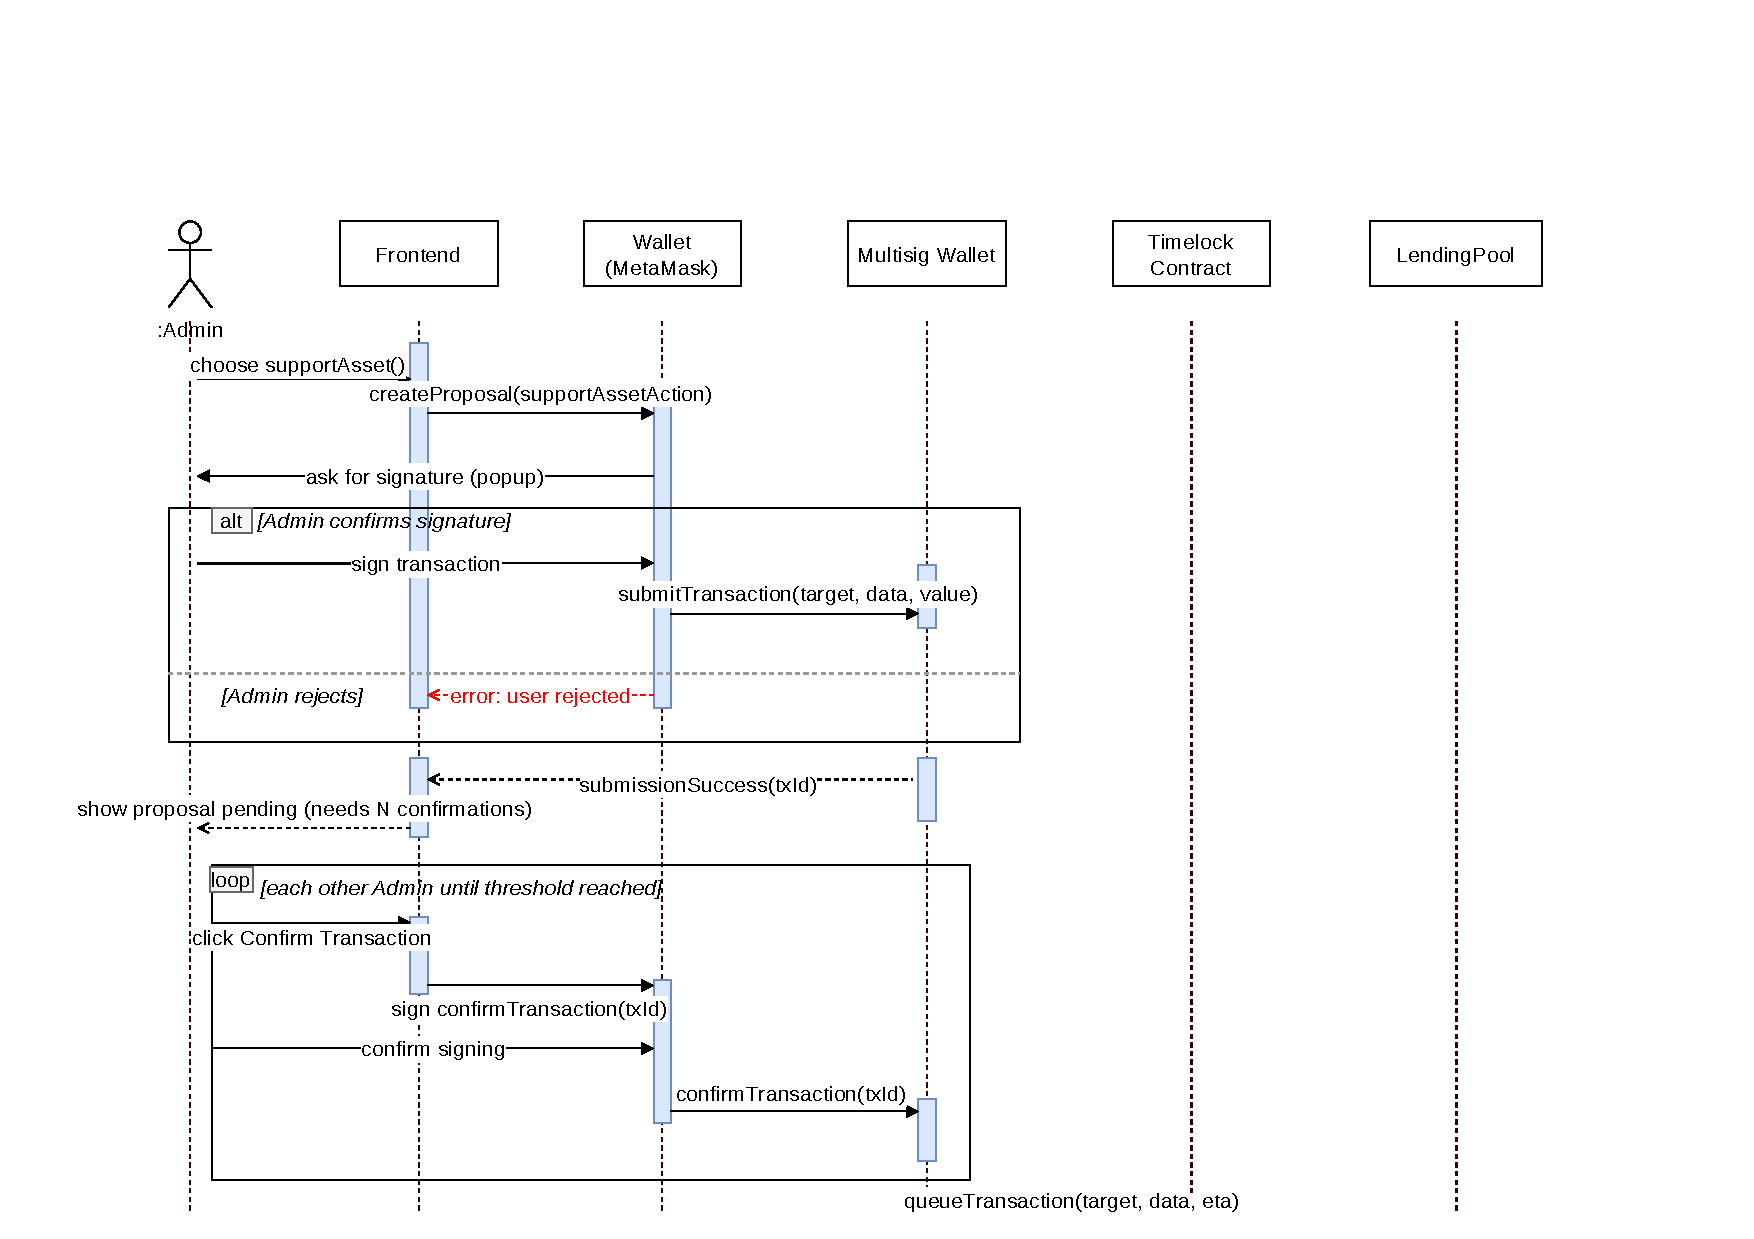
\includegraphics[
    page=1,
    width=\textwidth,
    height=0.9\textheight,
    keepaspectratio
]{../Hinhve/SSDHTTSM.pdf}

\vspace{0.5cm}

\includegraphics[
    page=2,
    width=\textwidth,
    height=0.9\textheight,
    keepaspectratio
]{../Hinhve/SSDHTTSM.pdf}

\caption{Sơ đồ tuần tự Hỗ trợ tài sản mới}
\label{fig:ssdhttsm}
\end{figure}

\section{Yêu cầu phi chức năng}


Bên cạnh các yêu cầu chức năng, hệ thống cần đáp ứng các yêu cầu phi chức năng sau: (i) Tính an toàn (Security): Giao thức phải đảm bảo an toàn trong việc quản lý tài sản của người dùng, ngăn chặn các truy cập trái phép, tấn công reentrancy, thao túng giá và các hành vi gây tổn hại đến hệ thống, (ii) Tính minh bạch (Transparency): Toàn bộ logic nghiệp vụ quan trọng được triển khai on-chain thông qua smart contract, cho phép bất kỳ ai cũng có thể kiểm tra và xác minh. (iii) Hiệu năng (Performance): Hệ thống cần đảm bảo khả năng hoạt động ổn định dưới số lượng giao dịch lớn, trong đó backend được sử dụng để index và truy vấn dữ liệu sự kiện. (iv) Khả năng mở rộng (Scalability): Thiết kế hệ thống cho phép dễ dàng mở rộng thêm tài sản mới, thay đổi mô hình lãi suất và nâng cấp giao thức trong tương lai.

\end{document}
